% !TeX root = ../main.tex
% Add the above to each chapter to make compiling the PDF easier in some editors.

\chapter{Base Operating System: Axcan OS}\label{chap:os}

In order to enable the proposed breathable distributed real-time system, capable of performing dynamic task migration across heterogenous embedded nodes, it is necessary that the nodes share a common software stack. The approach presented in this dissertation is based on a common lightweight and portable real-time operating system, which should fulfill some key requirements in order to be fit for the purpose. First, it should be lightweight enough to run on ECUs with constrained resources, as well as on containers that will act as digital twins of such ECUs but with possibly different resource and hardware sepcifications. Second, real-time behavior should be ensured for tasks on different criticality levels. Third, it should be able to execute precompiled applications which will be deployed dynamically, without the need for specific recompilation for each hardware platform. Existing operating systems often fall short on one or more of these requirements. For instance, lightweight real-time operating systems such as FreeRTOS offer low-overhead scheduling and real-time task management, but lack scheduling policies for mixed-criticality dynamic task loads, and do not offer dynamic task loading. On the other hand, more complex operating systems like Linux with Real-Time kernel might offer more flexible schedulers and dynamic application loading, but have a much larger OS footprint. Additionally, integration into the distributed system should be possible through the OS features to enable task migration and synchronization with other nodes.

This chapter presents Axcan OS, an operating system built as an extension to the microkernel of FreeRTOS and which builds the base behavior for ECU nodes to be integrated in the suggested approach. Axcan OS extended kernel provides an abstraction layer allowing for applications to run on multiple platforms in a seamless way, offering basic functionalities that enable the requirements mentioned before. The name of Axcan OS originates in the Nahuatl word \textit{axcan}, meaning "now" or "immediately", referring to the real-time capabilities of the system.

Axcan OS offers a few distinctive features that enable the breathable system proposed in this document. First of all, it includes a set of deployment management tasks, responsible for communicating with master node and controlling the execution of the tasks as instructed by master node. Second, it enables the dynamic execution of task applications (ELFs) on any compatible platform (sharing the same processor architecture), making it possible to execute exactly the same ELF file on virtual and physical nodes, independent of the rest of the underlying hardware and even software. Third, it offers a set of interfaces for system wide services, enabling the use of simple functionalities across all platforms. Finally, it implements further basic functionalities for real-time behavior, including a variety of real-time scheduling policies (some mixed-criticality capable) and time synchronization via PTP.

This chapter presents the details on the implementation and architecture of Axcan OS, along with some limitations in the scope of this work, but which are planned to be tackled in further development of the system.

\section{Architecture}
The architecture of Axcan OS is based on a microkernel, i.e. FreeRTOS, extending its core functionalities by a set of features as shown in Fig. \ref{fig:os_arch}.

\begin{figure}
	\centering
	\makebox[\textwidth]{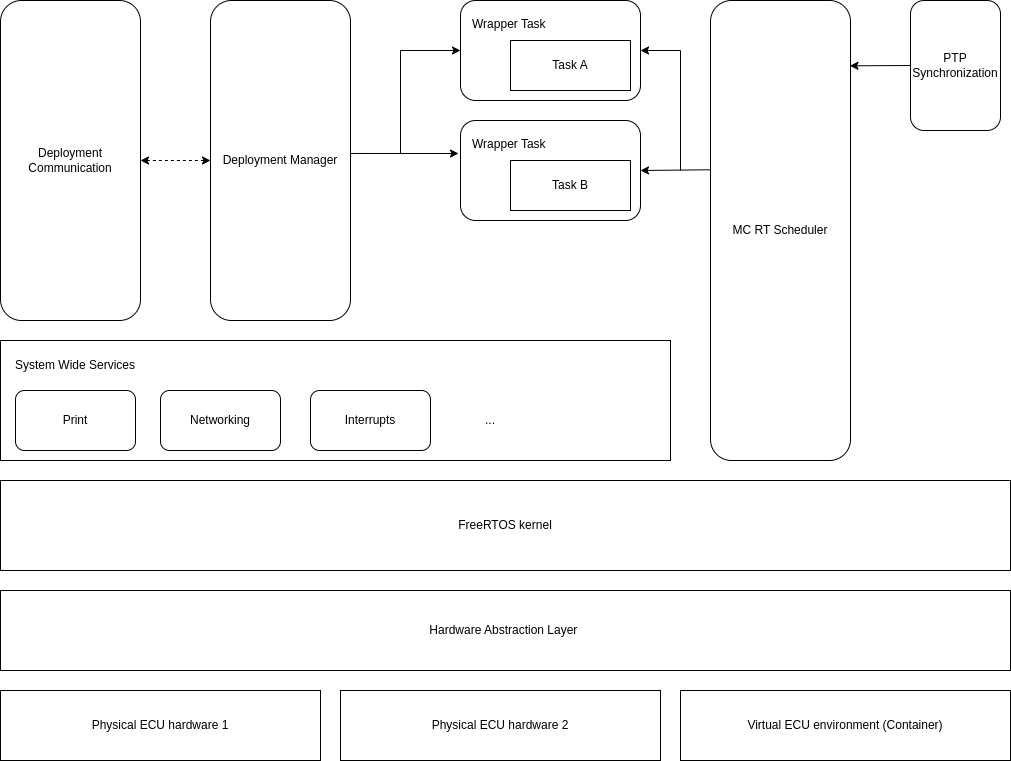
\includegraphics[width=\textwidth]{figures/os_arch_extended.png}}
	
	\caption{Axcan OS Architecture}
	\label{fig:os_arch}
\end{figure}

\begin{itemize}
	\item Extended Scheduler (Mixed Criticality and Real-Time Capable) - Based on ESFREE extension
	\item Task Deployment Communication Handler: Responsible for receiving instructions and task executables from a master node, as well as sending back messages about the status of the running system	
	\item Task Deployment Manager:  as well as triggering the dynamic control of the tasks (creation/destruction and start/stop/pause), as well as sending/receiving the checkpoint data. This includes the process of loading the ELF applications onto the system's memory.
	\item Wrapper Task: The user tasks, sent by the master node, shall be encapsulated in ELF files containing the machine code for them to run on top of the OS. However, as the core behavior of FreeRTOS does not contemplate loading of external applications, a wrapper task will allow for this feature. This wrapper task will handle some common functionalities for the user real-time tasks, such as: real-time constraint keeping, management of application stack and checkpoints, and passing handles for system functions to the applications
	\item System function services: these are services that are exposed to the user applications as "system functions". Since the microkernel architecture makes it tricky to handle some services globally by not offering shared libraries, some common functionalities (e.g. network communication or console prints) are offered by system services and passed via the wrapper task to the applications 
	\item PTP Synchronization: ensures the devices have a relatively small clock difference between each other, ensuring deadlines are relevant even when tasks are migrated
	\item FreeRTOS kernel and Hardware Abstraction Layer: ensure proper functioning and interfacing of basic system features and interfacing with hardware and peripherals
\end{itemize}

\section{Remote Task Deployment}
As an ECU represents a single node of the distributed system, and the execution of tasks is coordinated by the master node, Axcan includes a pair of tasks that act as an interface for deploying tasks remotely from the master node. First, the deployment communication thread is responsible for establishing a constant communication with the master node, exchanging status information about device health and current task load and status of each task. Also, this thread is responsible for receiving instructions from the master node regarding the execution of the assigned task set, which is then kept in a shared memory block and passed on to the deployment management thread. The deployment management thread is then responsible for handling the startup of the tasks and monitoring their status periodically. The startup includes first receiving the ELF and checkpoint files necessary for task execution, then allocating and initializing the memory required by the task, and finally creating the task thread and registering it in the mixed-criticality scheduler, which is then responsible for controlling when the CPU is given to the task. The monitoring sub-thread is then responsible for periodically checking whether the task is executing correctly, how many jobs have been executed, how many deadlines have been missed, etc. Furthermore, the monitoring is responsible also for pausing / stopping the tasks when told so by the master node, and for preparing and triggering the transfer of task files to another device when migration needs to occur.

\section{Mixed Criticality Scheduler}

The first step in achieving mixed criticality and respecting real-time behavior for the system applications is a scheduler that can achieve both goals. For this purpose, an extension of ESFREE (add reference), a project that implements a few dynamic and static real-time scheduling policies, including Earliest Deadline First (EDF), which for single core is ideally optimal (add references). This project is used as a base as the off-the-shelf FreeRTOS code only offers a priority-based scheduler, without any priority-assignment policies. In this work, the EDF policy is extended to cope with different levels of criticality by implementing the EDF with virtual deadlines for MC, as proposed in (add ref.).

**** Need to finalize implementing scheduling policies, then explain that into detail***

\section{Cross-Platform Task Loading}

To achieve the goal of executing the same application files on both physical and virtual ECU devices, the system integrates an ELF loader. This ELF loader, implemented to a great extent in collaboration with Yinbo Zhou in the scope of his master's thesis, enables the execution of multiple tasks, packed in the form of pre-compiled ELF files and with an additional data file. This approach tackles both challenges of allowing the dynamic loading of tasks and of stateful migration to the extent desired. In order for applications to be compatible with the task loader, they need to fulfill some requirements when compiled. The implemented loader is lightweight and meant to load the same application files on on multiple underlying hardware / software stacks, as shown in Fig. \ref{fig:multiplatform_tasks}, as long as an Axcan OS port runs on the target and the CPU architecture is the same as the target architecture for the compiled application, which in our case is always ARM Aarch64.


\begin{figure}
	\begin{minipage}{0.5\textwidth}
	\centering
	\makebox[0.9\textwidth]{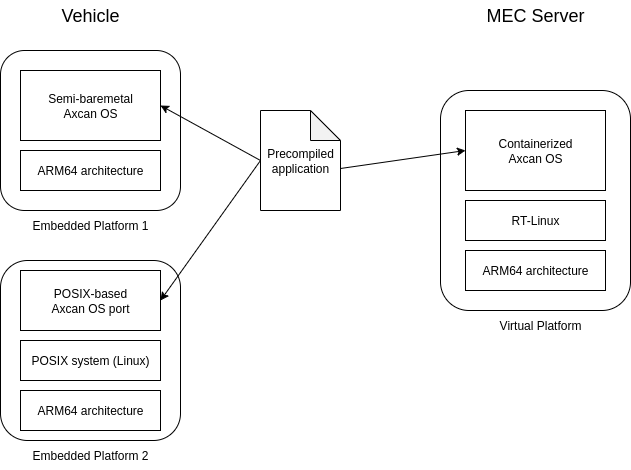
\includegraphics[width=0.9\textwidth]{figures/multiplatform_task_compatibility.png}}
	
	\caption{Cross-Platform Task Compatibility}
	\label{fig:multiplatform_tasks}
	\end{minipage}
	\begin{minipage}{0.5\textwidth}
	\centering
	\makebox[0.85\textwidth]{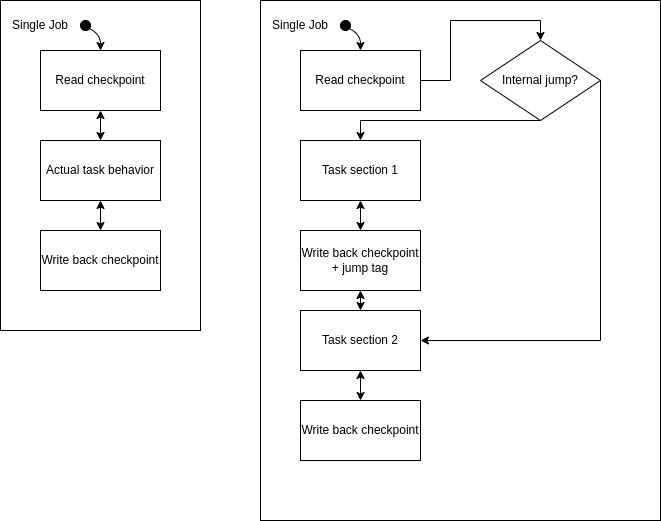
\includegraphics[width=0.85\textwidth]{figures/Task_arch.png}}
	
	\caption{User Application Flow}
	\label{fig:user_app_design}
	\end{minipage}
\end{figure}

\subsection{Hardware Abstraction Layer}
In order to achieve full compatibility across different platforms, an abstraction layer is added under Axcan OS. This layer ensures applications can run on any target platform independently of the hardware and software stack, apart from the architecture. The use of FreeRTOS kernel official ports already allows an abstraction layer in the form of FreeRTOS features, but due to the lightweight implementation of FreeRTOS, some features remain specific to the underlying platform, which is also undesired when aiming to load the same ELF file on different platforms. To achieve this, two core features are included as part of the extended kernel of Axcan OS. First, most of the system calls are encapsulated in wrappers, e.g.: the console output, network features, memory management, access to other peripherals, which are then offered via a standard signature that internally calls the proper underlying code. Second, the ELF loader, apart from processing the ELF and performing the needed relocations, needs to allocate memory for ELF execution, which should be aligned properly for the respective platform. This means that for hardware specific ports of FreeRTOS, which run on a bare metal system, memory can be allocated without any underlying considerations, but also requiring some memory management handling if no memory management unit (MMU) is available on the port. On the other hand, ports based on the POSIX port of FreeRTOS (e.g. the container approach running on a Linux server or even versions running as processes on top of UNIX based OSs) should take into consideration that the underlying OS is responsible for memory management, often not allowing standard \textit{malloc} calls to hold executable code. This specific case means that alternative memory allocation functions, such as \textit{mmap}, which are more flexible but require a more explicit memory handling in code, should be used. 


\subsection{User Application Requirements}
User applications need to meet two requirements to be compatible with Axcan OS. First, they need to be compiled with the right flags, particularly by enabling position independent execution (PIE) and to avoid integration of standard C libraries and system startup functions (they should use newlib to allow for applications to be encapsulated without dynamic library linking). Second, they should use the Axcan OS header and library files, which will provide access to basic system functions and core features, such as the checkpoint mechanism, the resource table for checkpoint variable handling and the proper entrypoint handling. System services are offered through global function pointers. All those elements are initialized by the operating system and passed to user applications through a data structure in shared memory.

Furthermore, by design user applications are periodic and must define and keep track of the state-relevant variables for their further execution, meaning that the main function acts as a single job execution, and any execution context needed for a job must be loaded at the beginning of the main and stored back at the end. This represents the minimal checkpoint version where state is only resumed from the beginning of a job. Further checkpoints can also be added in the middle of the code in the form of internal jumps that need to be executed at the start of the main function, allowing the job to resume also from internal points. These two cases are shown in Fig. \ref{fig:user_app_design}.

\subsection{Summary}
Axcan OS is an extended FreeRTOS kernel that enables the integration of embedded devices into the breathable distributed system proposed. Its core features make it possible to meet the functional requirements of 
